\section{Experiments}

\begin{figure}[t]
  \centering
  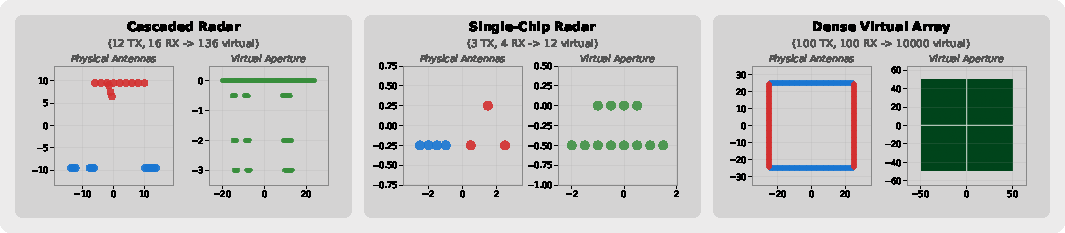
\includegraphics[width=\linewidth]{figs/antenna_layouts.pdf}
  \caption{Antenna configurations used in our evaluation. Left: cascaded MMWCAS-RF-EVM (12TX$\times$16RX $\to$ 86 unique azimuth virtual elements; Sec.~\ref{sec:supp_range_angle_resolution} in the supplement) used for training. Center: single-chip AWR1843 (3TX$\times$4RX $\to$ 12 virtual elements) used for cross-sensor transfer. Right: dense virtual array (100TX$\times$100RX $\to$ 10{,}000 virtual elements) used for 3D inference. Top row: physical TX (red) and RX (blue) positions. Bottom row: virtual aperture (TX$+$RX convolution).}
  \label{fig:antenna_layouts}
\end{figure}

We evaluate mmIR on seven diverse outdoor scenes from the ColoRadar dataset~\cite{kramer2022coloradar}, which provides synchronized mmWave radar and LiDAR captures with raw ADC access. We design three experiments that progressively test our forward model under increasingly challenging conditions: (1)~training evaluation on the cascaded imaging radar used for optimization (12TX$\times$16RX, 86 virtual elements); (2)~cross-sensor transfer to a co-located single-chip radar (3TX$\times$4RX, 12 virtual elements) without re-training; and (3)~3D occupancy inference via a dense virtual array (100TX$\times$100RX, 10{,}000 virtual elements). Figure~\ref{fig:antenna_layouts} illustrates all three antenna configurations. Dataset details, scene geometry reconstruction, and implementation hyperparameters are provided in the supplement (Sec.~\ref{sec:supp_implementation}).

\subsection{Training Evaluation: ADC Rendering and Range--Azimuth}
\label{sec:training_ra}

% Table 1: Training RA — Per-scene results with aggregate
\begin{table}[t]
\centering
\caption{Range--azimuth (RA) and ADC training evaluation across seven outdoor scenes. mmIR is compared against Sionna-RT~\cite{sionna}. Metrics: Pearson correlation (Corr), PSNR, SSIM, RMSE, and ADC-level magnitude error. Best in \textbf{bold}.}
\label{tab:training_ra}
\resizebox{\linewidth}{!}{%
\begin{tabular}{l cc cc cc cc cc cc}
\toprule
& \multicolumn{2}{c}{RA Correlation $\uparrow$} & \multicolumn{2}{c}{RA PSNR $\uparrow$} & \multicolumn{2}{c}{RA SSIM $\uparrow$} & \multicolumn{2}{c}{RA RMSE $\downarrow$} & \multicolumn{2}{c}{ADC Log-Mag MSE $\downarrow$} & \multicolumn{2}{c}{ADC MM-Mag MSE $\downarrow$} \\
\cmidrule(lr){2-3} \cmidrule(lr){4-5} \cmidrule(lr){6-7} \cmidrule(lr){8-9} \cmidrule(lr){10-11} \cmidrule(lr){12-13}
Scene & Ours & Sionna & Ours & Sionna & Ours & Sionna & Ours & Sionna & Ours & Sionna & Ours & Sionna \\
\midrule
  S0F135 & \textbf{0.921} & 0.418 & \textbf{37.4} & 21.4 & \textbf{0.938} & 0.509 & \textbf{0.0135} & 0.0850 & \textbf{48.3271} & 244.8361 & \textbf{0.0421} & 0.0469 \\
  S0F390 & \textbf{0.936} & 0.242 & \textbf{41.0} & 23.4 & \textbf{0.937} & 0.550 & \textbf{0.0089} & 0.0674 & \textbf{5.0250} & 294.3032 & \textbf{0.0289} & 0.0417 \\
  S1F185 & \textbf{0.954} & 0.312 & \textbf{39.8} & 18.9 & \textbf{0.926} & 0.326 & \textbf{0.0102} & 0.1138 & \textbf{32.3385} & 282.6453 & \textbf{0.0398} & 0.0461 \\
  S1F438 & \textbf{0.942} & 0.346 & \textbf{37.7} & 19.9 & \textbf{0.926} & 0.401 & \textbf{0.0130} & 0.1008 & \textbf{32.5274} & 288.9782 & \textbf{0.0369} & 0.0435 \\
  S2F105 & \textbf{0.887} & 0.188 & \textbf{34.6} & 28.7 & \textbf{0.894} & 0.724 & \textbf{0.0185} & 0.0367 & \textbf{23.5161} & 244.9075 & 0.0498 & \textbf{0.0481} \\
  S2F160 & \textbf{0.864} & 0.370 & \textbf{34.0} & 22.4 & \textbf{0.789} & 0.519 & \textbf{0.0200} & 0.0763 & \textbf{27.6683} & 275.3327 & \textbf{0.0444} & 0.0461 \\
  S2F300 & \textbf{0.930} & 0.388 & \textbf{38.7} & 21.3 & \textbf{0.906} & 0.512 & \textbf{0.0117} & 0.0858 & \textbf{30.0014} & 247.1371 & \textbf{0.0370} & 0.0543 \\
\midrule
  Mean & \textbf{0.919$\pm$0.030} & 0.324$\pm$0.076 & \textbf{37.6$\pm$2.4} & 22.3$\pm$3.0 & \textbf{0.902$\pm$0.049} & 0.506$\pm$0.115 & \textbf{0.0137$\pm$0.0038} & 0.0808$\pm$0.0229 & \textbf{28.4863$\pm$11.9698} & 268.3057$\pm$20.3703 & \textbf{0.0399$\pm$0.0061} & 0.0467$\pm$0.0037 \\
\bottomrule
\end{tabular}
}
\end{table}

\begin{figure}[t]
  \centering
  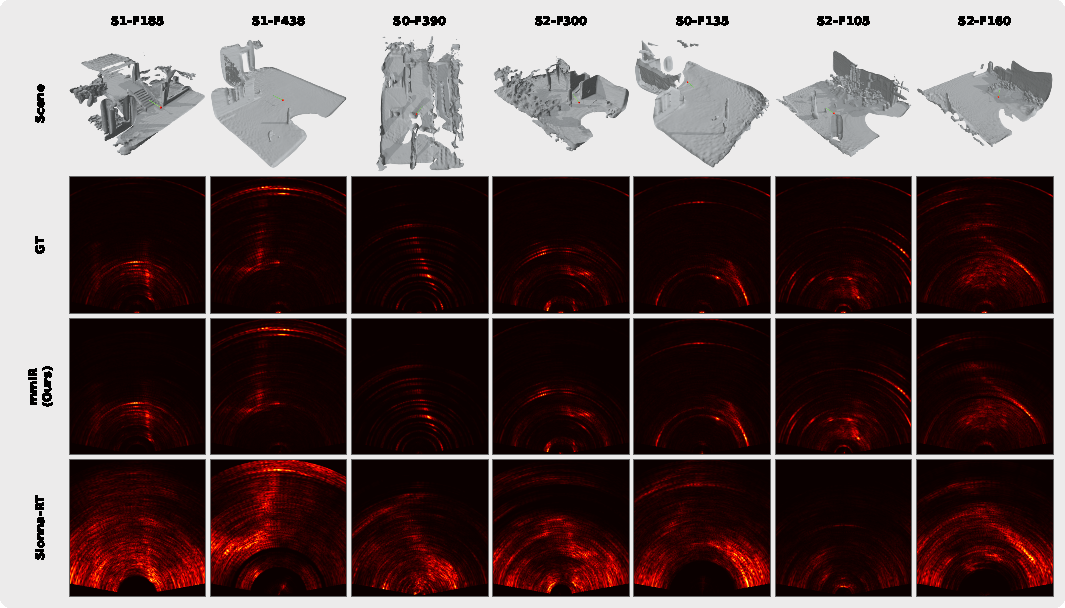
\includegraphics[width=\linewidth]{figs/training_ra/training_single_v2.pdf}
  \caption{Qualitative range--azimuth (RA) comparison across all seven training scenes, sorted by Pearson correlation (highest first). Each column shows one scene. Rows, top to bottom: scene mesh with radar position (red sphere) and boresight direction (green arrow); ground-truth RA; mmIR (ours); Sionna-RT baseline. Horizontal axis: cross-range (m); vertical axis: range (m). mmIR captures the dominant scatterer structure and multipath returns across all scenes, while Sionna-RT produces weaker, less spatially accurate responses.}
  \label{fig:eval_ra}
\end{figure}

We compare rendered and measured range--azimuth (RA) maps on the cascaded radar used for optimization. Table~\ref{tab:training_ra} reports Pearson correlation, PSNR, SSIM, RMSE, and ADC-level magnitude metrics across all seven scenes, with Sionna-RT~\cite{sionna} as baseline. Evaluating in the RA domain implicitly validates phase accuracy: the azimuth FFT converts relative phase differences across virtual elements into angular information, so any systematic phase error (per-element bias, incorrect path-length scaling, or incoherent phasor accumulation) would smear or shift targets in the angular domain, degrading all RA metrics. Absolute phase is not meaningful in practice, as it depends on user-configurable initial phase, oscillator drift, and phase noise; these common-mode offsets appear in the DC term of the spatial FFT and are dropped during processing.

mmIR achieves a mean Pearson correlation of \textbf{0.919}, substantially outperforming Sionna-RT (0.324). Table~\ref{tab:training_ra} quantifies this gap across all metrics; Figure~\ref{fig:eval_ra} provides the corresponding qualitative comparison, sorted by correlation. mmIR reproduces both the dominant scatterer locations and the diffuse multipath structure present in the ground truth, whereas Sionna-RT produces attenuated responses with spatially misaligned features.

Three architectural differences drive this gap. First, mmIR's physically-based BSDF with six per-vertex learnable parameters captures spatially varying reflectance that Sionna-RT's per-object scattering model cannot represent; this is most evident in geometrically complex scenes (S1-F438, S0-F135) where mixed-material surfaces dominate the radar response. Second, mmIR jointly optimizes surface normals and antenna beam patterns, parameters entirely outside Sionna-RT's optimization scope, correcting both surface orientation errors inherited from noisy LiDAR tessellation and systematic antenna gain biases. Third, Sionna-RT's path solver executes outside the AD graph: ray tracing runs under gradient suspension and all path geometry is subsequently detached, so while material gradients propagate through field coefficients at each bounce, the path topology itself is frozen and no gradients reach vertex positions or normals, and a material change at one surface cannot redirect subsequent bounces. mmIR places the entire forward model inside a single computation graph, enabling end-to-end gradient flow from the loss through ADC synthesis, phasor accumulation, BSDF evaluation, and ray--triangle intersections. The weakest scene, S2F160 (0.864), shows that even challenging geometries with complex multipath achieve high correlation. mmIR substantially outperforms the baseline on every scene, indicating that the richer parameter space and deeper gradient flow consistently improve fit quality.

\subsection{Radar Transfer Evaluation}
\label{sec:radar_transfer}

% Table 2: Radar Transfer — Per-scene results with aggregate
\begin{table}[t]
\centering
\caption{Cross-sensor transfer evaluation. Scene parameters optimized on the cascaded radar (12TX$\times$16RX, 86 unique azimuth virtual elements) are frozen and used to render ADC for the co-located single-chip radar (3TX$\times$4RX, 12 virtual elements) without re-training. Best in \textbf{bold}.}
\label{tab:radar_transfer}
\resizebox{\linewidth}{!}{%
\begin{tabular}{l cc cc cc cc cc cc}
\toprule
& \multicolumn{2}{c}{RA Correlation $\uparrow$} & \multicolumn{2}{c}{RA PSNR $\uparrow$} & \multicolumn{2}{c}{RA SSIM $\uparrow$} & \multicolumn{2}{c}{RA RMSE $\downarrow$} & \multicolumn{2}{c}{ADC Log-Mag MSE $\downarrow$} & \multicolumn{2}{c}{ADC MM-Mag MSE $\downarrow$} \\
\cmidrule(lr){2-3} \cmidrule(lr){4-5} \cmidrule(lr){6-7} \cmidrule(lr){8-9} \cmidrule(lr){10-11} \cmidrule(lr){12-13}
Scene & Ours & Bench. & Ours & Bench. & Ours & Bench. & Ours & Bench. & Ours & Bench. & Ours & Bench. \\
\midrule
  S0F135 & \textbf{0.533} & 0.002 & \textbf{25.6} & 17.8 & \textbf{0.505} & 0.464 & \textbf{0.0524} & 0.1283 & \textbf{10.9639} & 301.4341 & 0.2194 & \textbf{0.0668} \\
  S0F390 & \textbf{0.464} & 0.328 & 21.2 & \textbf{24.2} & 0.529 & \textbf{0.566} & 0.0873 & \textbf{0.0619} & \textbf{12.9644} & 331.2549 & \textbf{0.0630} & 0.0840 \\
  S1F185 & \textbf{0.567} & 0.136 & \textbf{22.4} & 20.1 & 0.422 & \textbf{0.480} & \textbf{0.0759} & 0.0990 & \textbf{0.5754} & 324.8441 & 0.1993 & \textbf{0.0771} \\
  S1F438 & \textbf{0.684} & 0.079 & \textbf{23.2} & 13.5 & \textbf{0.674} & 0.202 & \textbf{0.0694} & 0.2119 & \textbf{21.8672} & 348.0237 & 0.1507 & \textbf{0.0662} \\
  S2F105 & \textbf{0.608} & 0.084 & \textbf{24.7} & 22.8 & 0.609 & \textbf{0.690} & \textbf{0.0583} & 0.0721 & \textbf{3.4458} & 289.7929 & 0.1959 & \textbf{0.1068} \\
  S2F160 & \textbf{0.276} & 0.159 & \textbf{19.3} & 18.3 & \textbf{0.493} & 0.463 & \textbf{0.1085} & 0.1219 & \textbf{20.1530} & 338.1699 & 0.0893 & \textbf{0.0798} \\
  S2F300 & \textbf{0.745} & 0.008 & \textbf{27.2} & 23.6 & \textbf{0.468} & 0.412 & \textbf{0.0434} & 0.0661 & \textbf{7.7226} & 287.9379 & 0.1074 & \textbf{0.0948} \\
\midrule
  Mean & \textbf{0.554$\pm$0.143} & 0.114$\pm$0.103 & \textbf{23.4$\pm$2.5} & 20.0$\pm$3.6 & \textbf{0.529$\pm$0.080} & 0.468$\pm$0.138 & \textbf{0.0707$\pm$0.0206} & 0.1087$\pm$0.0488 & \textbf{11.0989$\pm$7.3886} & 317.3511$\pm$22.3659 & 0.1464$\pm$0.0565 & \textbf{0.0822$\pm$0.0136} \\
\bottomrule
\end{tabular}
}
\end{table}

A central claim of physics-based inverse rendering is that the optimized scene captures true physical properties, not sensor-specific patterns. We validate this by \emph{cross-sensor transfer}: the scene parameters trained on the cascaded radar (12TX $\times$ 16RX, 86 virtual elements) are frozen and used to render ADC for the single-chip radar (3TX $\times$ 4RX, 12 virtual elements) that shares the same physical mounting (Fig.~\ref{fig:antenna_layouts}). We apply the same rigid-body alignment transformation learned during cascaded training to the single-chip configuration and render forward-only.

This experiment tests whether our inverse renderer has learned transferable scene physics rather than memorizing the training sensor's idiosyncrasies. Table~\ref{tab:radar_transfer} shows that mmIR achieves a mean transfer correlation of \textbf{0.554}, outperforming Sionna-RT (0.114), demonstrating that the learned materials generalize across sensor configurations.

\subsection{Inference: 3D Occupancy via Dense Virtual Array}
\label{sec:3d_occupancy}

\begin{table}[t]
\centering
\caption{3D occupancy evaluation against LiDAR ground truth. Baseline: ColoRadar-provided 3D point cloud from the cascaded radar's near-1D virtual aperture, where elevation is synthesized by extruding range--azimuth detections along the vertical axis due to minimal elevation resolution. Ours: dense virtual array (100TX$\times$100RX) with full 2D aperture enabling range--azimuth--elevation (RAE) imaging. Occupancy metrics use KD-tree nearest neighbors ($\tau{=}0.5$\,m). Best in \textbf{bold}.}
\label{tab:3d_occupancy}
\resizebox{\linewidth}{!}{%
\begin{tabular}{l cc cc cc cc cc cc}
\toprule
& \multicolumn{2}{c}{Precision $\uparrow$} & \multicolumn{2}{c}{Recall $\uparrow$} & \multicolumn{2}{c}{F1 $\uparrow$} & \multicolumn{2}{c}{Accuracy $\uparrow$} & \multicolumn{2}{c}{RMSE $\downarrow$} & \multicolumn{2}{c}{R-CD $\downarrow$} \\
\cmidrule(lr){2-3} \cmidrule(lr){4-5} \cmidrule(lr){6-7} \cmidrule(lr){8-9} \cmidrule(lr){10-11} \cmidrule(lr){12-13}
Scene & Ours & ColoR & Ours & ColoR & Ours & ColoR & Ours & ColoR & Ours & ColoR & Ours & ColoR \\
\midrule
  S0F135 & 0.077 & \textbf{0.223} & 0.018 & \textbf{0.054} & 0.029 & \textbf{0.087} & 0.044 & \textbf{0.057} & \textbf{2.324} & 3.302 & 0.248 & \textbf{0.228} \\
  S0F390 & \textbf{0.481} & 0.045 & \textbf{0.110} & 0.014 & \textbf{0.179} & 0.021 & \textbf{0.212} & 0.017 & \textbf{2.692} & 2.745 & 0.216 & \textbf{0.207} \\
  S1F185 & \textbf{0.997} & 0.483 & \textbf{0.566} & 0.082 & \textbf{0.722} & 0.141 & \textbf{0.703} & 0.103 & \textbf{0.909} & 2.380 & \textbf{0.067} & 0.236 \\
  S1F438 & \textbf{0.633} & 0.433 & \textbf{0.265} & 0.117 & \textbf{0.373} & 0.185 & \textbf{0.362} & 0.131 & \textbf{1.511} & 3.339 & \textbf{0.116} & 0.268 \\
  S2F105 & \textbf{0.771} & 0.154 & \textbf{0.162} & 0.025 & \textbf{0.268} & 0.044 & \textbf{0.340} & 0.029 & \textbf{1.099} & 3.402 & \textbf{0.113} & 0.282 \\
  S2F160 & \textbf{0.516} & 0.383 & \textbf{0.177} & 0.165 & \textbf{0.264} & 0.231 & \textbf{0.257} & 0.183 & 1.917 & \textbf{1.611} & 0.146 & \textbf{0.118} \\
  S2F300 & \textbf{0.850} & 0.508 & \textbf{0.501} & 0.122 & \textbf{0.630} & 0.197 & \textbf{0.601} & 0.130 & \textbf{1.040} & 1.643 & \textbf{0.083} & 0.118 \\
\midrule
  Mean & \textbf{0.618$\pm$0.278} & 0.319$\pm$0.165 & \textbf{0.257$\pm$0.189} & 0.083$\pm$0.051 & \textbf{0.352$\pm$0.228} & 0.129$\pm$0.075 & \textbf{0.360$\pm$0.210} & 0.093$\pm$0.056 & \textbf{1.642$\pm$0.638} & 2.632$\pm$0.721 & \textbf{0.141$\pm$0.062} & 0.208$\pm$0.061 \\
\bottomrule
\end{tabular}
}
\end{table}

\begin{figure}[t]
  \centering
  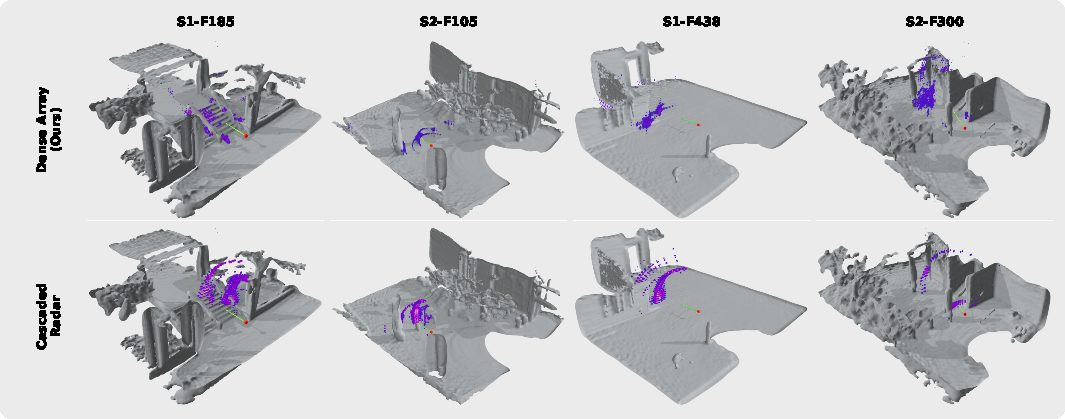
\includegraphics[width=\linewidth]{figs/test_3d/test_3d_v1.pdf}
  \caption{Single-frame 3D occupancy comparison overlaid on the LiDAR mesh. Top row: mmIR dense virtual array (100$\times$100 elements, uniform $\lambda/2$ spacing) with full 2D aperture enabling range--azimuth--elevation (RAE) imaging, thresholded at the 99.9th intensity percentile. Bottom row: ColoRadar-provided 3D point cloud from the cascaded radar's near-1D virtual aperture, which resolves only range--azimuth and extrudes detections along elevation, producing vertically smeared structure. Red sphere: radar position; green arrow: boresight direction.}
  \label{fig:3d_single_frame_comparison}
\end{figure}

After training, we freeze the optimized scene parameters and re-render from a dense virtual array (100TX $\times$ 100RX, 10,000 virtual elements with $\lambda/2$ spacing) inspired by the Rohde \& Schwarz QAR50~\cite{wirth2024maroon} (Fig.~\ref{fig:antenna_layouts}, right). We convert synthesized ADC into a 3D tensor via Range--Azimuth--Elevation (RAE) FFT and extract a sparse radar point cloud by thresholding at the 99.9th intensity percentile. Following~\cite{kung2025radarsplat}, we use single-bounce propagation at test time for the dense array.

We evaluate against LiDAR after radar-guided filtering: (1) filtering by the dense array's 0~dB beam limits, (2) projecting LiDAR points onto the radar polar voxel grid, and (3) retaining only points where radar normalized intensity $\geq 0.1$. Occupancy metrics use KD-tree nearest neighbors with $\tau=0.5$~m threshold; geometric fidelity is measured via RMSE and Relative Chamfer Distance (R-CD). Table~\ref{tab:3d_occupancy} shows substantial variation driven by radar visibility: scenes with multiple surfaces within the field-of-view achieve strong reconstruction (S1F185: Precision=0.997, R-CD=0.067), while open scenes with ground planes nearly parallel to boresight show degraded recall as specular energy is directed away from receivers. Additional qualitative analysis, quantitative ablation, and runtime results are in the supplement (Sec.~\ref{sec:supp_qualitative}).
